\documentclass[letterpaper,twocolumn,10pt]{article}
\usepackage{usenix2019_v3}
\usepackage{amsmath}
\usepackage{booktabs}
\usepackage{textcomp}
\usepackage{xurl}
\usepackage{graphicx}
\usepackage{tikz}
\usetikzlibrary{positioning,arrows.meta,fit}
\providecommand{\tightlist}{\setlength{\itemsep}{0pt}\setlength{\parskip}{0pt}}
\begin{document}
\date{}
\title{\Large \bf AttestRAG: End-to-End Attested Retrieval-Augmented Generation across CPU and GPU TEEs}
\author{{\rm Wei Wang}\\ \emph{affiliation to be added}}
\maketitle
{\small\noindent\emph{Draft v0.2, 2026-10-23. Wei Wang. Status markers: \textbf{[done]} = implemented and measured on hardware; \textbf{[design]} = designed, not implemented; \textbf{[TODO]} = open item for the next draft.}}
\begin{abstract}

Enterprises hand contracts, medical records and source code to retrieval-augmented generation (RAG) services, yet every deployed "confidential inference" offering protects only the model call: documents are parsed, embedded, indexed and retrieved in the clear on the provider\textquotesingle s host, and embeddings are not a safe intermediate form, since inversion attacks recover the text behind them. We present AttestRAG, a RAG system in which the whole pipeline, from parsing to generation, runs inside hardware-isolated confidential VMs, and in which a client can verify the entire chain before it uploads a single byte. AttestRAG binds the CPU TEE report, the GPU attestation and the measurement of every pipeline component into one composite statement; releases the keys that protect the persisted vector index only after a small, pure policy function accepts that statement; and seals every answer with a one-time key that only the attested node can learn, so that neither the host nor the network can forge or swap a reply. We built AttestRAG on AMD SEV-SNP with a reproducible, measured boot chain (firmware, kernel, initrd, command line and a dm-verity root filesystem under one launch measurement), attached an NVIDIA H200 in confidential-computing mode to the same VM, and evaluated it end to end on the RGB benchmark. Attestation is not the cost: establishing a verified session takes 10--30 ms with the CPU report alone and about 65 ms with the GPU transcript as well, far below a single answer. Retrieval inside the TEE loses nothing (hit@4 = 1.0 on both languages). CPU-bound generation sets a latency floor of 1.4 s per English answer and 3.2 s per Chinese answer and collapses under concurrency; the same pipeline with the confidential GPU answers in 0.17 s and 0.28 s and serves 8 users at 7 answers per second, 25x the CPU throughput, with the GPU\textquotesingle s firmware measurements pinned by the same policy. The verifier, policy engine and key-release protocol are 2.6 k lines of Python with no dependency beyond a cryptography library, small enough that the release protocol can be analysed as a whole and the policy function run as an executable specification.

\end{abstract}

\section{Introduction}\label{introduction}

RAG has become the default way to put private corpora in front of a large language model. The corpus is parsed into chunks, each chunk is embedded into a vector, the vectors are indexed, and at query time the nearest chunks are retrieved and pasted into the model prompt. Every one of these stages sees the customer\textquotesingle s data in plaintext, and every one of them typically runs on infrastructure the customer does not control.

The industry\textquotesingle s answer has been confidential inference: run the model inside a trusted execution environment (TEE), attest it, and call it over an encrypted channel. This protects exactly one stage. The parser, the embedding model, the vector database and the retriever remain outside the enclave, on the provider\textquotesingle s host, where the host operating system, the hypervisor and the operator can read them. Nor is the vector representation a form of protection: few-shot embedding-inversion attacks such as ALGEN reconstruct the original text from a handful of vectors \cite{chen2025algen}. Cryptographic RAG proposals go the other way: RemoteRAG \cite{cheng2025remoterag} hides the user\textquotesingle s query behind differential-privacy noise and partially homomorphic distance computation, and SAG \cite{zhou2025sag} encrypts chunks and vectors before they are stored, with a formal proof. Neither protects the generation step, where the retrieved plaintext meets the model, and both pay for the cryptography on every query.

Two things make a different design possible now. First, CPU TEEs that isolate a whole virtual machine (AMD SEV-SNP, Intel TDX) are generally available, and a recent evaluation measured LLM inference under TDX at under 10 \% overhead, H100 confidential mode at 4--8 \%, and a complete RAG pipeline (Elasticsearch, BM25, SBERT) inside TDX at 6--7 \% \cite{chrapek2025confidential}. Second, NVIDIA\textquotesingle s Hopper and Blackwell GPUs offer a confidential-computing mode with their own attestation. What is missing is a system that puts the complete pipeline inside these TEEs and, more importantly, lets a client verify the complete pipeline as one object. The gap is not academic: the TEE.fail authors observed that NVIDIA does not bind an H100\textquotesingle s attestation to the identity of the VM it serves, so an attacker can forward the GPU report of another machine \cite{chuang2025teefail}.

This paper presents AttestRAG, a RAG system with the following properties.

\begin{itemize}
\tightlist
\item
  \textbf{Everything inside.} Parsing, embedding, the vector index, retrieval and generation run in confidential VMs. The vector database keeps its storage on a tmpfs inside encrypted guest memory; the only thing that reaches the host disk is an authenticated-encrypted snapshot.
\item
  \textbf{One composite proof.} The CPU report carries, in its \texttt{report\_data}, a hash of a session nonce and of an ephemeral public key generated inside the TEE; every GPU report of the session carries a hash of that CPU \texttt{report\_data}. The launch measurement covers firmware, kernel, initrd, command line and, through a dm-verity root hash on the command line, every byte of the root filesystem, including the models and the vector database binary.
\item
  \textbf{Keys only after proof.} A key broker service (KBS) outside the provider\textquotesingle s trust domain releases the index key wrapped to the TEE\textquotesingle s ephemeral key only after cryptographic verification of the composite evidence and after a policy decision that includes a measurement allow-list, a component-wise minimum TCB and the guest-policy bits of the VM.
\item
  \textbf{Client-side verifiability.} The client SDK runs the same verifier and the same policy as the KBS, before it uploads anything. Questions are encrypted to the attested node key and carry a one-time reply key, and the answer is sealed with that key, so an answer the client accepts can only have been produced by the node that could read the question.
\end{itemize}

We implemented AttestRAG (Section 7) and deployed it on a self-hosted SEV-SNP machine (2x AMD EPYC 9554, 4x H200 NVL) with a reproducible image build whose measurement we verify offline. Section 8 reports the first end-to-end measurements on the RGB benchmark \cite{chen2024rgb}. The GPU stage is implemented and measured on one H200 in confidential mode. The Intel TDX verifier and the formal analysis of the release protocol are designed but not yet implemented; the paper marks these parts explicitly, and Appendix A lists the status of every claim.

\textbf{Contributions.}

\begin{enumerate}
\def\labelenumi{\arabic{enumi}.}
\tightlist
\item
  A threat model and design for a RAG system in which no pipeline stage runs outside a TEE and the cloud operator and the service provider are both untrusted (Sections 4--5). \textbf{{[}done{]}} for the CPU pipeline.
\item
  A composite attestation protocol that binds the CPU report, the GPU reports and the pipeline measurement into one verifiable statement, closing the GPU-report-forwarding gap (Section 5.2). \textbf{{[}done{]}}: the CPU half, the binding rule and the NVIDIA verifier, exercised against a real H200 transcript.
\item
  Post-attestation key release with a measurement allow-list, component-wise minimum TCB and guest-policy checks, and an index that is sealed per tenant and never present in plaintext on the host (Section 5.3--5.4). \textbf{{[}done{]}}; rollback protection \textbf{{[}design{]}}.
\item
  A key-release protocol and policy designed for formal analysis: the protocol properties that matter (a key reaches only the TEE that proved possession in the same session; no replay; no cross-session GPU evidence) are stated for a symbolic protocol model, and the policy function is small, total and pure so that its executable specification can be the engine that actually runs (Section 6). \textbf{{[}done{]}} for the code; the protocol model and the executable specification are \textbf{{[}TODO{]}}.
\item
  An open-source implementation and an end-to-end evaluation on real SEV-SNP hardware with a confidential H200, including the attestation and key-release costs, retrieval and answer quality inside the TEE, and the concurrency behaviour of CPU-only against confidential-GPU inference (Sections 7--8). \textbf{{[}done{]}}.
\end{enumerate}

\section{Background}\label{background}

\textbf{VM-level TEEs.} AMD SEV-SNP and Intel TDX isolate an entire guest VM from the hypervisor: guest memory is encrypted with a per-VM key, integrity is protected (reverse map table on SNP, TD-owner bits on TDX), and the platform security processor signs an attestation report on request. An SNP report (version 5 on current firmware) contains the launch measurement, a 64-byte \texttt{report\_data} field chosen by the guest, the guest policy bits (debug, migration agent, SMT, \ldots{}), the current and reported TCB (bootloader, TEE, SNP firmware and microcode security version numbers), the chip identifier and a signature by the chip\textquotesingle s VCEK, whose certificate chains to AMD\textquotesingle s ASK and ARK. The launch measurement is computed over the initial memory image: with OVMF and the \texttt{kernel-hashes} feature it covers the firmware, the kernel, the initrd and the kernel command line \cite{amd2024snpabi}.

\textbf{GPU confidential computing.} NVIDIA Hopper and Blackwell GPUs can run in a confidential mode in which a single GPU is passed through to a confidential VM, the PCIe link is protected by an SPDM session, device memory is encrypted and the GPU produces an attestation report over its firmware measurements, verifiable against NVIDIA\textquotesingle s attestation service \cite{nvidia2024cc}. A reverse-engineering study of this mode found that over a thousand BAR0 register fields remain host-readable and that RPC metadata is in plaintext with timing side channels \cite{gu2025nvidiacc}. The report does not by itself say which VM the GPU is attached to; binding it to the CPU report is the system\textquotesingle s job (Section 5.2).

\textbf{RAG pipeline and what each stage exposes.} Ingest parses documents into chunks (plaintext documents). Embedding turns chunks into vectors (plaintext chunks in, invertible vectors out). The vector index stores vectors and the chunk text as payload (both). Retrieval embeds the query and runs nearest-neighbour search (the query, the access pattern over the index). Generation puts the query and the retrieved chunks into one prompt (everything). A design that protects only generation therefore still leaks the corpus, the index and the queries.

\textbf{Remote attestation and key brokers.} The IETF RATS architecture \cite{rfc9334} separates the attester, the verifier and the relying party. In confidential-container deployments the relying party is a key broker service (Trustee KBS in Confidential Containers \cite{trustee}) that releases secrets only to attested workloads. AttestRAG follows this structure with its own small reference KBS, so that the complete release path can be read and, later, formalized.

\section{Motivation and problem analysis}\label{motivation-and-problem-analysis}

\textbf{Where inference-only TEEs leak.} Consider the common deployment: a vector database and an embedding service on ordinary hosts, and a model served from a confidential VM behind an attested TLS endpoint. The host of the vector database sees every chunk in plaintext as payload and every query as a vector and as text (the embedding service receives the raw query). The embedding host sees every document. Only the prompt-to-answer leg is protected, and that leg contains nothing the earlier legs have not already exposed. Encrypting the index at rest with a key held by the database host changes nothing, since the host holds the key.

\textbf{GPU report forwarding.} A GPU attestation report proves that \emph{some} GPU with the stated firmware is in confidential mode. If the relying party accepts it alongside a CPU report without a cryptographic link between the two, an operator can run the model on an ordinary GPU and present the report of a confidential GPU elsewhere. This is exactly the gap TEE.fail reported for H100 \cite{chuang2025teefail}. The verifier rejects a real H200 transcript replayed under another session\textquotesingle s \texttt{report\_data} (Section 8.6); \textbf{{[}TODO{]}}: reproduce the forwarding with a second confidential GPU on another machine.

\textbf{Why not cryptographic RAG.} Differentially private and homomorphic retrieval \cite{cheng2025remoterag} protects the query against the index host, and encrypted storage \cite{zhou2025sag} protects the index at rest, but both still deliver plaintext chunks to a generation step that must see them; the generator is then the weak point, and the per-query cryptographic cost grows with the index. A TEE design pays a near-constant overhead instead and protects the generator too.

\section{Threat model and security goals}\label{threat-model-and-security-goals}

\textbf{Assets.} Customer documents, chunks, embeddings, the vector index, queries, answers, and the data-encryption key (DEK) that seals the index.

\textbf{Trusted.} The CPU TEE hardware and firmware at or above the minimum TCB named in the policy (the AMD secure processor and SEV firmware; the TDX module once supported); the GPU confidential-computing firmware when a GPU is used; the measured AttestRAG VM image; the KBS, operated by the customer or a party the customer trusts; and the client SDK.

\textbf{Untrusted.} The cloud provider\textquotesingle s host OS, hypervisor and operators; storage and the network; other tenants; and the AttestRAG operator when it is not the customer. The adversary can read, modify and replay anything on disk or on the network; boot a modified image; enable debug; run on an outdated, vulnerable TCB; and replay old evidence or splice evidence from a different VM, session or GPU.

\textbf{Goals.} (G1) Confidentiality of documents, vectors, queries and answers against everything untrusted. (G2) Integrity of retrieval results and answers: a client accepts an answer only if it was produced by the attested node over the question the client sent. (G3) Client-side verifiability: a client can establish G1 and G2 before uploading, with no trust in the provider.

\textbf{Out of scope.} Physical attacks on memory, such as the DDR5 interposer of TEE.fail \cite{chuang2025teefail} and the sub-\$50 DDR4 interposer of Battering RAM \cite{demeulemeester2026batteringram}, are excluded by the hardware vendors\textquotesingle{} threat model and by ours; firmware attacks on the AMD secure processor \cite{shen2026aspbreaker} and the SEV-SNP memory-consistency attacks of \cite{schlueter2026fabricked,zhang2026stackwarp,schlueter2026staleus,schlueter2025heracles} are the reason the policy carries a minimum TCB; microarchitectural side channels and the access pattern of nearest-neighbour search over the index are only partly mitigated and are discussed in Section 9; availability is not a goal. What the model \emph{says} is not a security property: documents can carry prompt injections and a small model will follow them; AttestRAG grounds answers in retrieved chunks and citations but does not make the model honest.

\section{System design}\label{system-design}

\subsection{Architecture}\label{architecture}

\begin{figure*}[t]\centering
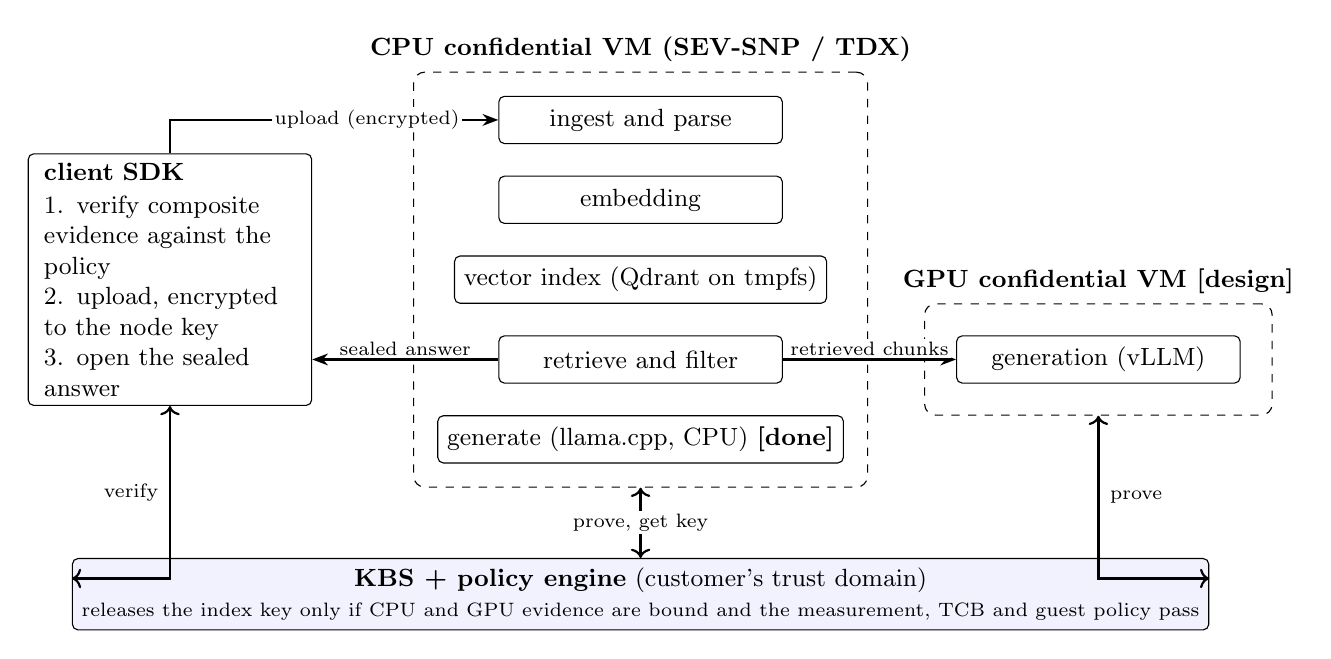
\begin{tikzpicture}[font=\small, node distance=4mm,
  stage/.style={draw, rounded corners=2pt, minimum width=3.6cm, minimum height=6mm, align=center, fill=white},
  vm/.style={draw, dashed, rounded corners=4pt, inner sep=3mm},
  arr/.style={-{Stealth[length=2mm]}, thick}, lbl/.style={font=\scriptsize, fill=white, inner sep=1pt}]
  \node[stage] (ingest) {ingest and parse};
  \node[stage, below=of ingest] (embed) {embedding};
  \node[stage, below=of embed] (index) {vector index (Qdrant on tmpfs)};
  \node[stage, below=of index] (retrieve) {retrieve and filter};
  \node[stage, below=of retrieve] (gen) {generate (llama.cpp, CPU) \textbf{[done]}};
  \node[vm, fit=(ingest)(gen), label={[font=\small\bfseries]above:CPU confidential VM (SEV-SNP / TDX)}] (cpuvm) {};
  \node[stage, right=22mm of retrieve] (gpugen) {generation (vLLM)};
  \node[vm, fit=(gpugen), inner sep=4mm, label={[font=\small\bfseries]above:GPU confidential VM \textbf{[design]}}] (gpuvm) {};
  \node[stage, left=18mm of index, text width=3.2cm, minimum height=22mm, align=left]
    (client) {\textbf{client SDK}\\[1pt] 1. verify composite evidence against the policy\\ 2. upload, encrypted to the node key\\ 3. open the sealed answer};
  \node[stage, fill=blue!5, minimum width=9cm, minimum height=9mm, below=12mm of gen, align=center]
    (kbs) {\textbf{KBS + policy engine} (customer's trust domain)\\ \scriptsize releases the index key only if CPU and GPU evidence are bound and the measurement, TCB and guest policy pass};
  \draw[arr] (client.north) |- (ingest.west) node[lbl, pos=0.8] {upload (encrypted)};
  \draw[arr] (retrieve.west) -- (client.east |- retrieve.west) node[lbl, midway, above] {sealed answer};
  \draw[arr] (retrieve.east) -- (gpugen.west) node[lbl, midway, above] {retrieved chunks};
  \draw[arr, <->] (cpuvm.south) -- (kbs.north -| cpuvm.south) node[lbl, midway] {prove, get key};
  \draw[arr, <->] (gpuvm.south) |- ([yshift=2mm]kbs.east) node[lbl, pos=0.25, anchor=west, xshift=1mm] {prove};
  \draw[arr, <->] (client.south) |- ([yshift=2mm]kbs.west) node[lbl, pos=0.25, anchor=east, xshift=-1mm] {verify};
\end{tikzpicture}
\caption{One composite proof covers the whole pipeline: the SNP report of the VM and the attestation transcript of the GPU attached to it. The node proves itself to the KBS before it receives any key; the client verifies the same composite evidence before it uploads.}\label{fig:arch}
\end{figure*}

Figure~\ref{fig:arch} shows the architecture. The CPU confidential VM runs the ingest parser, the embedding model, the vector database (Qdrant) with its storage on a tmpfs inside guest memory, the retriever and the generator (a small instruction-tuned model served by llama.cpp, on the GPU when one is attached and on the CPU otherwise, from the same measured binaries). A GPU in confidential-computing mode is passed through to this VM rather than to a VM of its own: the PCIe link carries an SPDM session between the guest driver and the GPU, device memory is encrypted, and DMA goes through bounce buffers in guest memory. Because the GPU\textquotesingle s own report does not say which VM it serves (Section 3), keeping the GPU inside the attested VM puts the driver that owns the SPDM session into the measured image and makes the GPU report part of the VM\textquotesingle s session rather than a second party\textquotesingle s. All of these are files in a read-only root filesystem whose dm-verity root hash is part of the launch measurement (Section 5.5), so replacing the embedding model, the vector database binary or the node\textquotesingle s Python code changes the measurement and the KBS refuses the key. The node exposes three operations over JSON/HTTP: \texttt{attestation(nonce)}, \texttt{ingest(doc\_id,\ wrapped\_document)} and \texttt{query(wrapped\_question)}.

\subsection{Composite attestation}\label{composite-attestation}

Every session starts with a 32-byte nonce from the verifier (the KBS, or the client). The node generates an ephemeral X25519 key pair inside the TEE and asks the platform for a report over

\begin{footnotesize}
\begin{align*}
\mathit{rd}_{\mathrm{cpu}} &= \mathrm{SHA\text{-}384}(\ell_{\mathrm{cpu}} \parallel \mathit{nonce} \parallel \mathit{pk}_{\mathrm{tee}})\\
\mathit{rd}_{\mathrm{gpu}} &= \mathrm{SHA\text{-}384}(\ell_{\mathrm{gpu}} \parallel \mathit{rd}_{\mathrm{cpu}})
\end{align*}
\end{footnotesize}

with the labels \(\ell_{\mathrm{cpu}}\) = \texttt{attestrag-rd-v1}, \(\ell_{\mathrm{gpu}}\) = \texttt{attestrag-gpu-bind-v1} and length-prefixed concatenation, so that no choice of a shorter nonce and a longer key can collide with another pair. \texttt{report\_data} is the 64-byte field of the report that the guest chooses (offset 0x50 of an SNP report; a SHA-384 digest fills 48 bytes); the platform signs it together with the measurement and the TCB, so whatever is written there is bound to this chip and this launch.

The CPU rule binds two things. The \emph{nonce} is a 32-byte random value from the verifier, single-use and expiring after 60 s: a report whose \texttt{report\_data} matches it was produced in this session and cannot be a replay. This matters because SNP reports carry no timestamp; freshness rests entirely on the nonce. The \emph{public key} is generated inside the TEE for this session and its private half never leaves it: the KBS wraps the DEK to that key, so a man-in-the-middle who relays a genuine report cannot open the key it obtains, and one who substitutes its own key breaks the hash and with it the signature. Together the rule states one fact, proved once: \emph{this} TEE, in \emph{this} session, holds the private key.

The GPU rule hangs every GPU report of the session off the CPU report: a GPU report carries not an independent nonce but the hash of the CPU \texttt{report\_data}. The composite verifier therefore verifies the CPU evidence first, derives the expected GPU \texttt{report\_data} from it, and only then verifies each GPU evidence. A GPU report is valid for exactly one CPU report, hence one session. This is the check that closes the forwarding gap of Section 3: a confidential GPU\textquotesingle s report taken from another machine or another session fails the \texttt{report\_data} comparison, whatever its own signature says. The two rules yield one statement for the policy engine: \emph{this CPU TEE (measurement M, TCB T) holds sk in this session, and these GPUs attested for it in the same session}; the policy never judges a GPU on its own.

What the binding does not prove: the GPU rule establishes session freshness, not that the GPU is the one physically attached to this VM over an SPDM-protected link. Closing that requires the VM to attest its own GPU session, for example a measured driver placing the SPDM session identity in the CPU report, and is left for the GPU stage. \textbf{{[}done{]}}: the rule, the composite verifier and the NVIDIA verifier. The latter parses the SPDM GET\_MEASUREMENTS transcript that the driver returns through NVML (the 37-byte request followed by the signed MEASUREMENTS response), chains the GPU\textquotesingle s attestation-key certificate through NVIDIA\textquotesingle s provisioning and identity certificates to the pinned NVIDIA Device Identity CA, verifies the ECDSA P-384 signature over request and response, compares the \emph{request} nonce with \texttt{gpu\_report\_data} (the response nonce is chosen by the GPU, as SPDM specifies, so freshness comes from the signed request half of the transcript), checks the firmware identifier in the certificate\textquotesingle s DICE extension against the one the report carries, and reduces the 64 DMTF measurement blocks to one SHA-384 digest that the policy pins. A transcript captured from the H200 inside the confidential VM is a golden test. Reference-measurement lookup (NVIDIA\textquotesingle s RIM service) and certificate revocation, which NVIDIA\textquotesingle s own verifier adds, are \textbf{{[}design{]}}.

\textbf{What the SNP verifier checks.} Parse the version-5 report; reject VLEK-signed reports (not yet supported) and unknown signature algorithms; derive the product (Milan, Genoa, Turin) from the CPUID family and model in the report and refuse a mismatch with the configured product; fetch AMD\textquotesingle s ARK and ASK for that product from the bundled copies and compare the ARK against a pinned public key; fetch the VCEK for the chip identifier and reported TCB from AMD\textquotesingle s key distribution service, caching it on disk; verify the chain ARK $\rightarrow$ ASK $\rightarrow$ VCEK and the certificates\textquotesingle{} validity window; check that the VCEK\textquotesingle s hardware-identifier extension equals the report\textquotesingle s \texttt{CHIP\_ID} and that its SPL extensions equal the report\textquotesingle s \texttt{REPORTED\_TCB}; verify the ECDSA P-384 signature over the report; and compare \texttt{report\_data} against the expected value. The verifier then emits claims: platform, measurement, decoded TCB components, debug flag, guest policy, launch TCB and signer identity.

\subsection{Key hierarchy and release}\label{key-hierarchy-and-release}

The KBS holds, per tenant, the index DEK. \textbf{{[}design{]}}: a tenant master key that wraps per-index DEKs, and per-session keys derived for the client channel; the current implementation has one DEK per key identifier. The release protocol is:

\begin{enumerate}
\def\labelenumi{\arabic{enumi}.}
\tightlist
\item
  the node requests a challenge and receives a single-use nonce with a 60 s lifetime;
\item
  the node generates the ephemeral key pair, obtains the composite evidence over \texttt{cpu\_report\_data(nonce,\ pub)} and sends \texttt{(key\_id,\ nonce,\ pub,\ evidence)};
\item
  the KBS consumes the nonce (even on failure), verifies the evidence, evaluates the policy, writes an audit record, and only on \texttt{allow} returns the DEK wrapped to \texttt{pub} with X25519 ECDH, HKDF-SHA256 (salt = both public keys, info = a versioned label and the key identifier) and AES-256-GCM;
\item
  the node unwraps the DEK in TEE memory and opens the sealed index.
\end{enumerate}

\textbf{Policy.} The verifier establishes that the evidence is genuine; the policy turns that into a decision that the machine is worth trusting. It is the customer\textquotesingle s own statement, evaluated independently by the KBS and by the client with the same rules, that only a TEE running the named image, on firmware at or above a named version and without debug enabled, may receive a key. A policy is a plain record: allowed CPU platforms, a measurement allow-list, a component-wise minimum TCB (bootloader, TEE, SNP firmware, microcode), the allowed guest-policy values (for example \texttt{0x30000}, which forbids debug and the migration agent and fixes the ABI version), whether debug is allowed, a freshness window, and the same fields for GPUs. Evaluation is a total function from policy and claims to a decision with a list of reasons; \texttt{allow} holds if and only if the list is empty. The TCB comparison is component-wise and never lexicographic: a newer microcode does not compensate for an older SNP firmware.

\subsection{Persisted index}\label{persisted-index}

The vector database runs with its storage directory on a tmpfs, so vectors and chunk text exist only in encrypted guest RAM. After each ingest the node asks the database for a collection snapshot, seals it with the DEK under AES-256-GCM with the format version, the collection name and the vector dimension as associated data, and writes it to an untrusted data disk provided by the host. At start the node unseals the snapshot in memory and restores the collection through the database\textquotesingle s upload interface, so plaintext never touches a file. A host that edits, truncates or swaps the file gets an authentication failure and the node refuses to start. \textbf{{[}done{]}}. The snapshot is whole-collection, so sealing costs O(index) per ingest; incremental sealing or a dm-crypt volume keyed by the KBS is future work. Rollback to an older, validly sealed snapshot is detected only when the KBS also tracks a monotonic index version \textbf{{[}design{]}}; permission-aware retrieval (filtering by the caller\textquotesingle s rights inside the TEE) and multi-tenancy are \textbf{{[}design{]}}.

\subsection{Measured image and boot chain}\label{measured-image-and-boot-chain}

The guest image is built reproducibly: a golden qcow2 image is shrunk to a minimal ext4 root, a dm-verity hash tree is computed with a fixed salt, and two consecutive builds are byte-identical. The VM boots OVMF with \texttt{kernel-hashes} enabled, so the launch measurement signed by the platform covers the firmware, the kernel, the initrd and the command line; the command line carries \texttt{roothash=\textless{}dm-verity\ root\ hash\textgreater{}}, so every block of the root filesystem is transitively under the measurement. Guest writes go to a tmpfs overlay and are lost at reboot; persistent state exists only through the attested KBS and index path. The expected measurement is computed offline with \texttt{sev-snp-measure} \cite{sevsnpmeasure} from the firmware, kernel, initrd, command line, vCPU count and vCPU model, and equals the value the platform signs. The policy JSON is never part of the image, since it would have to contain its own measurement; the verifier side supplies it.

\subsection{Client SDK and answer authenticity}\label{client-sdk-and-answer-authenticity}

The client runs the same verifier and policy as the KBS. \texttt{connect()} draws a nonce, requests the node\textquotesingle s evidence and its transport public key, verifies the evidence against \texttt{cpu\_report\_data(nonce,\ node\_pub)}, evaluates the policy, and only then remembers \texttt{node\_pub}; any call before a successful \texttt{connect()} is refused locally. Documents are wrapped to \texttt{node\_pub} with the document identifier as context. A question is wrapped together with a freshly drawn one-time reply key; the node\textquotesingle s answer, including the retrieved hits and citations, is sealed under that reply key with a fixed associated-data label. An adversary on the network or on the host can neither read the question nor produce an answer the client will accept, because learning the reply key requires the node\textquotesingle s private transport key, which exists only inside the attested VM. An earlier design that returned answers in plaintext was forgeable on the network; this version fixes it.

\section{\texorpdfstring{Formal analysis of key release \textbf{{[}design{]}}}{Formal analysis of key release {[}design{]}}}\label{formal-analysis-of-key-release-design}

Where formal methods earn their place here is the release protocol, not the policy function. The policy function is under a hundred lines of set membership and integer comparison; a proof that it satisfies its own rules would mostly restate it. None of the defects found while building the system were in it: the launch-TCB field read at the wrong offset, the certificate parser rejecting AMD\textquotesingle s zero serial numbers, and an earlier answer path that a network adversary could forge all sat in the verifier, the parser and the protocol. The analysis is therefore split into two parts with different tools, and the paper states what neither covers.

\textbf{Protocol properties.} The release protocol of Section 5.3 together with the binding rules of Section 5.2 forms a small protocol between a TEE, a KBS and a network adversary who controls the host. The properties the system relies on are protocol properties with an adversary, and they will be stated and checked in a symbolic model (Tamarin or ProVerif):

\begin{itemize}
\tightlist
\item
  \textbf{Possession}: if the KBS releases a key wrapped to a public key \(pk\), then a TEE that passed verification and policy generated \(pk\) and holds the matching private key; an adversary who relays genuine evidence obtains nothing it can open.
\item
  \textbf{Freshness}: a release is preceded by a challenge in the same session; evidence from an earlier session, or evidence replayed after its nonce was consumed, is never accepted.
\item
  \textbf{No cross-session GPU evidence}: a GPU report accepted with a CPU report was produced over that CPU report\textquotesingle s \texttt{report\_data}; a report from another machine or session is rejected whatever its own signature says. This is the forwarding gap of Section 3, stated as a property.
\item
  \textbf{Answer authenticity}: an answer the client accepts was produced by the node that decrypted the question, since the reply key travels only inside the question wrapped to the node\textquotesingle s attested key.
\end{itemize}

The model abstracts the hardware signature as an unforgeable signature by the chip and treats the verifier as correct; it will not find a parsing bug, a wrong reference value in the policy, or a side channel.

\textbf{Executable policy specification.} The policy function, \texttt{evaluate(policy,\ claims,\ now)}, is total, pure and operates on frozen records of strings and integers, and it is the one piece that must agree exactly between the KBS and every client. It will be written once in Lean 4 with a few algebraic theorems (monotonicity: enlarging an allow-list or lowering a minimum TCB can only turn denials into releases, never the reverse; component-wise TCB: a shortfall in any component implies denial whatever the other components; debug or an unlisted guest policy implies denial), and the usual objection, that the verified model is not the code that runs, is removed by running it: Lean 4 compiles to a native binary, and the KBS and the client SDK will call that binary as the policy engine. Until then the Python function and the Lean function are kept in agreement by differential testing over generated policies and claims (the test suite already enumerates every denial reason). The trusted computing base for release decisions is then the verifier (signature and chain checks, 450 lines of Python), the policy specification and the KBS loop (60 lines).

\textbf{{[}TODO{]}}: the symbolic model and its results; the Lean specification with its line counts and proof sizes; the differential-test harness.

\section{Implementation}\label{implementation}

\begin{figure*}[t]
\centering
\includegraphics[width=\textwidth]{figures/architecture.pdf}
\caption{The deployed system on h200: one attested Python process (node, attester, KBS client), three local services inside the measured VM, the sealed snapshot on the untrusted disk, and the KBS in the customer\textquotesingle s trust domain.}\label{fig:impl}
\end{figure*}

AttestRAG is about 2,600 lines of Python 3.11 in nine modules (attest, policy, kbs\_client, ingest, embed, index, retrieve, generate, sdk) plus the node and the two HTTP services, with 1,300 lines of tests (74 tests, including a real Genoa report and VCEK verified against AMD\textquotesingle s pinned roots and a real H200 attestation transcript verified against NVIDIA\textquotesingle s, plus a bound SNP+GPU pair as the composite golden case) and 800 lines of deployment shell. The NVIDIA attester is 30 lines over NVML; the verifier is 150 lines and needs nothing from NVIDIA\textquotesingle s SDK. The only runtime dependencies are \texttt{cryptography} and \texttt{numpy}. The SNP attester uses the kernel\textquotesingle s configfs-tsm interface and needs no vendor tool inside the guest; the verifier bundles AMD\textquotesingle s root certificates and fetches VCEKs from AMD KDS with an on-disk cache. The HTTP transport is JSON over the standard library (no TLS yet: metadata such as document identifiers and sizes is visible on the wire). Generation and embedding use llama.cpp\textquotesingle s server \cite{llamacpp} with Qwen3-Embedding-0.6B (Q8\_0, 1024 dimensions) and Qwen2.5-Instruct in Q4\_K\_M, the 1.5B model for the CPU-only configuration and the 7B model once the GPU is attached (both files are in the image; which one the chat server loads is part of the measurement); the vector database is Qdrant 1.19 \cite{qdrant} accessed over its REST API. All binaries and model weights are pinned by SHA-256 in the image build.

The self-hosted deployment runs QEMU 11.1 built from source (distribution packages lacked SEV-SNP guest support) with OVMF.amdsev from Ubuntu\textquotesingle s 2025.11 build; the Ubuntu 24.04 firmware (2024.02) fails to boot under upstream QEMU SNP. The guest is a 32-vCPU, 16 GB SEV-SNP VM; the vCPU count is part of the measurement. The image is 12.4 GB with both generators and boots unattended into attest $\rightarrow$ key release $\rightarrow$ serve. An end-to-end script runs 34 checks against the live VM: SNP active, dm-verity root bound to the expected root hash, the platform-signed measurement equal to the offline value, key release allowed under the published policy and denied with a wrong measurement and with a minimum TCB above the platform\textquotesingle s, the client refusing to upload to a node whose measurement is not in its policy, and the sealed snapshot restoring the index after a restart.

The GPU is one of the host\textquotesingle s four H200 NVL, switched to confidential mode with NVIDIA\textquotesingle s administration tool and passed to the VM with VFIO over iommufd (the legacy VFIO container caps DMA mappings at 65,535, too few for a guest whose memory flips between private and shared page by page). Four things stood between a working GPU and the first CUDA call, none of them in the attestation path: a 1 TB 64-bit MMIO window made the firmware spend over fifteen minutes in its page tables (512 GB, enough for the GPU\textquotesingle s 256 GB BAR, boots in seconds); the GPU had to sit behind a PCIe root port with a link speed, since on the root bus the driver reports an unknown link rate and CUDA refuses to initialise although attestation works; the distribution\textquotesingle s kernel-module package needs its module index rebuilt in the image; and CUDA stays disabled until the guest sets the GPU\textquotesingle s ready state, which a unit now does before the servers start. Detaching the GPU from the host was the only step that touched the host\textquotesingle s other workloads: every CUDA process opens every GPU\textquotesingle s device node, so the driver cannot release one GPU until all of them restart.

Two implementation findings in the verifier are worth recording. The launch-TCB field sits at offset 0x1F0 of a version-5 report, not 0x1F8 as an earlier draft assumed; the real report caught it. And AMD\textquotesingle s VCEK certificates carry serial number 0, which recent versions of the \texttt{cryptography} library deprecate; the verifier loads them explicitly so that a future hard rejection fails loudly in the golden test rather than silently in production.

\section{Evaluation}\label{evaluation}

The evaluation answers three questions: what attestation and key release cost; whether moving the whole pipeline into the TEE loses retrieval or answer quality; and where the time goes. All measurements are from the self-hosted machine (2x EPYC 9554 Genoa, SEV firmware 1.55, 32-vCPU SEV-SNP guest), through the attested client path: the CPU-only configuration on 2026-10-20 (Sections 8.3--8.4) and the same image with the confidential H200 attached on 2026-10-23 (Section 8.5). \textbf{{[}TODO{]}}: the comparison against an unprotected deployment and against an inference-only TEE deployment, larger indexes and a second CPU platform (TDX) are not yet measured; the 10 \% end-to-end overhead target of the outline remains a target, not a result.

\subsection{Benchmark and method}\label{benchmark-and-method}

We use RGB \cite{chen2024rgb}, a bilingual benchmark for RAG with 300 English and 300 Chinese news questions, each with positive passages that contain the answer, negative passages on the same topic without the answer, and answer aliases. For 100 sampled questions per language we ingest one document per question holding its positive and negative passages shuffled (median 24 passages); for a held-out 20 \% the positives are omitted, so the corpus contains on-topic noise but no answer. Each question is asked once with k = 4. Retrieval is scored as hit@4 (a retrieved chunk shares a 120-character window with a positive passage), answers with RGB\textquotesingle s alias match, and rejection by a phrase list in both languages. A concurrency sweep then runs N clients, each with its own attested session, over 16 questions never asked before, since llama.cpp caches prompt prefixes and repeated questions would measure the cache.

\subsection{Attestation and key release}\label{attestation-and-key-release}

Establishing a verified session, which is an SNP report through configfs-tsm, the certificate-chain and signature checks with the cached VCEK, and the policy evaluation, takes 10--30 ms on the client (median 12 ms across 64 sessions in the sweep). The first contact with a chip and TCB adds one fetch from AMD KDS, after which the VCEK is cached. Key release at node start is one such round trip plus the unsealing of the snapshot. With the GPU attached the session also carries the SPDM transcript and its five-certificate chain; verifying them adds about 35 ms (65 ms per session in the GPU sweeps). Per-user attestation is therefore free compared with one answer on the CPU and about a third of one on the GPU.

\subsection{Retrieval and answer quality inside the TEE}\label{retrieval-and-answer-quality-inside-the-tee}

Table~\ref{tab:quality} shows the results.

\begin{table}[t]\centering\small\setlength{\tabcolsep}{4pt}
\begin{tabular}{p{1.55in}ll}\toprule
 & \textbf{Chinese} & \textbf{English} \\ \midrule
corpus (100 documents) & 814 chunks & 3,762 chunks \\
hit@4 & 1.00 & 1.00 \\
positive chunks among the 4 (mean) & 3.2 & 3.1 \\
answer accuracy (RGB alias match) & 0.94 & 0.96 \\
false rejection on answerable questions & 0.00 & 0.00 \\
held out: rejection ("context insufficient") & 0.05 & 0.05 \\
\bottomrule\end{tabular}
\caption{Retrieval and answer quality on RGB inside the SEV-SNP VM (100 questions per language: 80 answerable, 20 held out; k = 4).}\label{tab:quality}
\end{table}

Retrieval through the encrypted index and the in-TEE vector database loses nothing: a positive passage is among the four retrieved chunks for every question, in a corpus where two thirds of the passages are on-topic noise. The remaining answer errors are the 1.5B generator picking the wrong fact out of a correct context. The weak point is negative rejection: when the answer is absent from the corpus the model refuses only 5 \% of the time and otherwise answers from pretraining or fabricates. This is the behaviour the RGB authors report even for ChatGPT; for AttestRAG it means that the generator, not the TEE, bounds answer trustworthiness, and that a production node needs a larger model or a relevance gate that refuses when no chunk passes a similarity threshold. Rejection rate should be reported as a security-relevant metric alongside accuracy.

\subsection{Latency and throughput}\label{latency-and-throughput}

Table~\ref{tab:latency} gives the single-user latencies.

\begin{table}[t]\centering\small\setlength{\tabcolsep}{4pt}
\begin{tabular}{p{1.45in}ll}\toprule
\textbf{single user, client side} & \textbf{Chinese} & \textbf{English} \\ \midrule
ingest, per document (median 24 passages), p50 / p90 & 4.5 s / 5.9 s & 6.1 s / 8.6 s \\
ingest throughput & 1.8 chunks/s & 6.2 chunks/s \\
answer (embed + search + generate), p50 / p90 & 3.2 s / 3.7 s & 1.4 s / 1.7 s \\
\bottomrule\end{tabular}
\caption{Single-user latency measured at the client, including the network hop into the guest.}\label{tab:latency}
\end{table}

Chinese is slower because the same 800-character chunk is about three times as many tokens: the prompt is around 2,000 tokens against 700 for English, and CPU prompt processing runs at about 700 tokens per second on 32 vCPUs. Ingest time is embedding plus the whole-collection sealed snapshot after every document, so it grows with the collection. For calibration, the first configuration of the same VM (8 vCPUs, 2 embedding threads, 6 generation threads) ingested 0.31 chunks/s and answered a Chinese question in 10.3 s; the vCPU count and the thread counts are part of the measured image, so the change was a rebuild with a new expected measurement.

Table~\ref{tab:sweep} shows the sweep.

\begin{table*}[t]\centering\small\setlength{\tabcolsep}{4pt}
\begin{tabular}{lrlrlr}\toprule
\textbf{users} & \textbf{English q/s} & \textbf{English p50 / p90} & \textbf{Chinese q/s} & \textbf{Chinese p50 / p90} & \textbf{errors} \\ \midrule
1 & 0.60 & 1.4 s / 2.7 s & 0.36 & 3.1 s / 3.5 s & 0 \\
2 & 0.21 & 8.9 s / 16.4 s & 0.18 & 12.5 s / 16.7 s & 0 \\
4 & 0.23 & 17.4 s / 25.6 s & 0.17 & 17.6 s / 35.8 s & 0 \\
8 & 0.29 & 26.5 s / 39.5 s & 0.24 & 34.3 s / 47.6 s & 0 \\
\bottomrule\end{tabular}
\caption{Concurrency sweep: $N$ clients, each with its own attested session, 16 unseen questions per level.}\label{tab:sweep}
\end{table*}

Throughput drops three-fold as soon as two users overlap and does not recover: the inference server runs four slots on a unified KV cache and interleaves the prompts, while the embedding server and the generation server, 32 threads each, run at the same time on 32 vCPUs and oversubscribe them. (With the inference server\textquotesingle s default 4,096-token cache the same sweep failed outright for two or more users with KV-cache allocation errors; a 16k cache removed the errors but not the slowdown.) None of this is attestation cost; it is CPU inference, and it is the quantitative motivation for the GPU stage: prompt processing at 700 tokens per second is the whole budget, and a GPU in confidential mode does the same work in milliseconds, as the next section measures.

\subsection{The confidential GPU configuration}\label{the-confidential-gpu-configuration}

The same image, corpus and questions with GPU3 of the host passed through in confidential-computing mode and both llama.cpp servers on the CUDA build with every layer offloaded. The policy now requires GPU evidence and pins the composite digest of the GPU\textquotesingle s 64 firmware measurements, so every session in this table verified an H200 transcript as well as an SNP report.

Table~\ref{tab:gpu} gives the numbers.

\begin{table}[t]\centering\small\setlength{\tabcolsep}{4pt}
\begin{tabular}{p{1.6in}p{0.95in}p{0.95in}}\toprule
 & \textbf{Chinese} & \textbf{English} \\ \midrule
verified session (SNP report + GPU transcript + policy) & 0.07 s & 0.06 s \\
answer accuracy (RGB alias match) & 0.95 & 0.975 \\
hit@4 / false rejection / held-out rejection & 1.00 / 0.00 / 0.05 & 1.00 / 0.00 / 0.05 \\
answer, single user, p50 / p90 & 0.28 s / 0.34 s & 0.17 s / 0.21 s \\
2 users: q/s, p50 / p90 & 5.0, 0.37 s / 0.57 s & 1.7, 0.39 s / 6.9 s \\
4 users: q/s, p50 / p90 & 3.7, 0.57 s / 2.1 s & 6.7, 0.58 s / 0.83 s \\
8 users: q/s, p50 / p90 & 6.7, 1.07 s / 1.34 s & 7.1, 1.04 s / 1.29 s \\
\bottomrule\end{tabular}
\caption{The confidential GPU configuration: same image and corpus, H200 NVL in CC mode attached to the VM, both llama.cpp servers on CUDA.}\label{tab:gpu}
\end{table}

An answer is 8x (English) to 11x (Chinese) faster than on 32 vCPUs and eight users get 25x the CPU throughput (7.1 against 0.29 answers per second), because generation now runs at 330--390 tokens per second and prompt processing is no longer the budget; what remains per answer is retrieval plus a few hundred milliseconds of generation. The language gap shrinks from 2.3x to 1.6x since the longer Chinese prompts are cheap on the GPU. Quality is unchanged, the models being the same, and so is the negative-rejection weakness with the 1.5B model (the 7B model below changes that). The two p90 outliers (6.9 s at two users, 2.1 s at four) are single slow requests, not errors. The confidential-mode overhead of the GPU itself is not separated here: the same build on an unprotected H200 was not measured in this round, and the 4--8 \% that \cite{chrapek2025confidential} and \cite{ibarra2025ccgpu} report for Hopper is below the noise of a 100-question sample. What the table does show is the cost of the composite proof: about 30 ms per session for the GPU half, against answers of 170--280 ms.

The spare device memory also pays for the generator the CPU could not afford. With Qwen2.5-7B-Instruct in place of the 1.5B model (same quantisation, 7.7 GB of device memory), negative rejection, the weak spot of Section 8.3, rises from 5 \% to 35 \% of the held-out questions in both languages and Chinese answer accuracy to 0.99, at 2.5x the single-user latency and half the 8-user throughput, both still an order of magnitude inside the CPU-only envelope. 35 \% is not yet a safe gate; a relevance threshold or a verifier pass remains necessary, but it is now a filter on top of a model that does refuse, not a substitute for one.

Table~\ref{tab:model} compares the two generators.

\begin{table}[t]\centering\small\setlength{\tabcolsep}{4pt}
\begin{tabular}{p{1.2in}p{1.05in}p{1.05in}}\toprule
 & \textbf{1.5B (zh / en)} & \textbf{7B (zh / en)} \\ \midrule
answer accuracy & 0.95 / 0.975 & 0.99 / 0.975 \\
held out: rejection & 0.05 / 0.05 & 0.35 / 0.35 \\
false rejection & 0.00 / 0.00 & 0.00 / 0.025 \\
answer p50 / p90 & 0.28 / 0.34 s, 0.17 / 0.21 s & 0.62 / 0.87 s, 0.46 / 0.63 s \\
8 users: q/s & 6.7 / 7.1 & 2.6 / 3.6 \\
\bottomrule\end{tabular}
\caption{Generator size on the confidential GPU: Qwen2.5-1.5B against Qwen2.5-7B (both Q4\_K\_M), same image family, corpus and questions.}\label{tab:model}
\end{table}

\subsection{Security checks}\label{security-checks}

The end-to-end suite exercises the negative paths on the live VM: a policy with a different measurement makes the client refuse to upload (exit 3) and makes the KBS deny the key with the reason \texttt{measurement\ not\ in\ allow-list}; a minimum SNP firmware version one above the platform\textquotesingle s is denied with \texttt{tcb\ \textquotesingle{}snp\textquotesingle{}=24\ \textless{}\ required\ 25}; a guest-policy allow-list of \texttt{0x20000} denies the \texttt{0x30000} VM; flipping one bit in the report\textquotesingle s policy or measurement field breaks the signature; flipping one bit in the reported TCB breaks the match against the VCEK\textquotesingle s SPL extensions; a report for a different nonce fails the \texttt{report\_data} check; and a sealed snapshot with one byte changed, the wrong key, or the wrong collection name in the associated data fails authentication and the node refuses to start. For the GPU half, the real H200 transcript is rejected by the unit tests when presented under another session\textquotesingle s \texttt{report\_data} (the forwarding case of Section 3), with one bit of the measurement record changed, with a certificate chain that does not end in the pinned NVIDIA root, or with a firmware identifier that differs between certificate and report. \textbf{{[}TODO{]}}: a live forwarding test between two machines, and index rollback once the version counter exists.

\section{Discussion and limitations}\label{discussion-and-limitations}

\textbf{Physical and side-channel attacks.} DDR interposer attacks \cite{chuang2025teefail,demeulemeester2026batteringram} break the hardware assumption of every VM-level TEE and are out of scope; a platform whose firmware has a published arbitrary-code-execution bug \cite{shen2026aspbreaker} is excluded by the minimum-TCB check only once a fixed firmware exists and the policy names it. Access-pattern leakage of nearest-neighbour search inside the VM (page faults, cache, the ciphertext side channels of \cite{schlueter2025heracles}) could reveal which chunks a query touches; ORAM-style indexing is a possible mitigation at a cost we have not measured. On the GPU side, the host-readable registers and plaintext RPC metadata documented in \cite{gu2025nvidiacc} remain even when the GPU stage exists.

\textbf{Single GPU and what the GPU proof does not say.} The implementation passes one GPU through to one confidential VM; multi-GPU confidential computing (NVLink, SPDM across devices) is a later tier. The GPU transcript proves that a GPU with the pinned firmware is in confidential mode and answered this session\textquotesingle s nonce; it does not prove that the SPDM session the driver holds terminates at that GPU, which would need the measured driver to place the session identity in the CPU report. The verifier also pins the firmware digest itself rather than consulting NVIDIA\textquotesingle s reference-measurement service, so a firmware update is a policy change, and it does not check revocation. Memory swapping under confidential mode, where PipeLLM measured up to 88 \% throughput loss and recovered most of it with speculative pipelined encryption \cite{tan2025pipellm}, did not arise here because the models fit in device memory.

\textbf{Key management.} The reference KBS keeps keys in memory and in a 0600 JSON file, has one policy for all keys, no rotation or revocation, no durable audit log, no TLS and no client authentication; a deployment would use Trustee or an HSM-backed broker with the same protocol. Freshness relies entirely on the single-use nonce, since SNP reports carry no time. VLEK-signed reports and Intel TDX evidence are not yet verified.

\textbf{Model behaviour.} The TEE guarantees what code ran and what data it saw, not that the model told the truth. Section 8.3 shows a 1.5B model fabricating answers when the corpus has none; prompt injection through documents is likewise outside the TEE\textquotesingle s reach.

\section{Related work}\label{related-work}

\textbf{Confidential inference.} Measurements of LLM inference under VM TEEs agree that the model call itself is cheap: under 10 \% on TDX and 4--8 \% on H100 confidential mode \cite{chrapek2025confidential}, 1--3 \% on B200 with TDX when configured correctly and 30--40 \% with default settings \cite{asad2026blackwell}, with a systematic H100 study in \cite{ibarra2025ccgpu}. The same ETH Zurich study also ran a RAG pipeline inside TDX at 6--7 \% overhead \cite{chrapek2025confidential}, as an evaluation rather than a system: it does not attest the pipeline or bind its components. EnclaveX \cite{schambach2026enclavex} is the closest system: TDX confidential VMs with H200 confidential GPUs orchestrated by Kubernetes and SCONE, with keys released only after a unified attestation, at about 1.3 \% attestation overhead; it does not cover retrieval, and its attestation is an orchestration-level property rather than something the end client verifies. PipeLLM \cite{tan2025pipellm} reduces the cost of encrypting swapped GPU memory under H100 confidential mode. AttestRAG differs in scope (the whole RAG pipeline, including the index and its persistence), in the composite proof, and in the client-side verifiability of the complete chain.

\textbf{TEE attacks.} TEE.fail \cite{chuang2025teefail} uses a DDR5 bus interposer costing under \$1,000 to extract Intel\textquotesingle s provisioning key, forge TDX attestations and steal ECDSA keys from SEV-SNP VMs, and it is also the source of the GPU-report-forwarding observation that Section 5.2 addresses. Battering RAM \cite{demeulemeester2026batteringram} does the same on DDR4 for under \$50 against SGX and patched SEV-SNP platforms. ASPBreaker \cite{shen2026aspbreaker} achieves arbitrary code execution on the AMD secure processor from an old firmware version and shows that the compromise carries over to newer versions, decrypting VM memory and forging reports; Fabricked, StackWarp and STALEUS \cite{schlueter2026fabricked,zhang2026stackwarp,schlueter2026staleus} and Heracles \cite{schlueter2025heracles} attack SEV-SNP through Infinity Fabric misconfiguration, memory inconsistency and chosen plaintexts. Together they define the boundary of our threat model and motivate the component-wise minimum-TCB check, which is the only defence a relying party has against firmware with known vulnerabilities, and the explicit exclusion of physical access. For the GPU, \cite{gu2025nvidiacc} documents the host-visible state that remains under confidential mode.

\textbf{Cryptographic and private RAG.} RemoteRAG \cite{cheng2025remoterag} protects the user\textquotesingle s query with differential privacy and partially homomorphic encryption, not the document store; SAG \cite{zhou2025sag} encrypts chunks and vectors before storage and proves security formally; ALGEN \cite{chen2025algen} shows why vectors need protecting at all. Surveys of RAG security \cite{mu2026securerag,palanisamy2026ragsp} catalogue poisoning and injection, which are orthogonal to the confidentiality problem addressed here. Commercial confidential-AI offerings (Opaque, Phala, Fortanix) are not described in enough detail to compare.

\section{Conclusion}\label{conclusion}

AttestRAG shows that a RAG pipeline can run entirely inside confidential VMs and be verified as one object by the party whose data it handles. On real SEV-SNP hardware with a confidential H200, attestation and key release cost tens of milliseconds per session, retrieval inside the TEE is lossless, generation on the confidential GPU answers in a few hundred milliseconds, and the measured boot chain plus the pinned GPU firmware digest turn every pipeline component into a policy decision. What remains is binding the GPU\textquotesingle s SPDM session into the VM\textquotesingle s report, the formal analysis of the release protocol, and the comparison against unprotected and inference-only deployments that will decide whether the end-to-end overhead target holds.

\appendix

\section{Claim status}\label{claim-status}

Table~\ref{tab:status} lists every claim with its status.

\begin{table*}[t]\centering\small\setlength{\tabcolsep}{4pt}
\begin{tabular}{p{2.6in}p{1.3in}p{2.45in}}\toprule
\textbf{Claim or component} & \textbf{Status} & \textbf{Evidence} \\ \midrule
Whole CPU pipeline inside a measured SEV-SNP VM & done & deploy/h200, e2e 34/34 \\
SNP verifier (chain, hwID, SPL, signature, report\_data) & done & tests with a real Genoa report \\
Composite CPU + GPU binding rule and verifier & done & real H200 transcript + synthetic chain tests \\
Key release after proof; measurement, min-TCB, guest-policy checks & done & KBS audit, e2e deny cases \\
Index sealed with AEAD, never plaintext on host & done & Qdrant on tmpfs + sealed snapshots \\
Index rollback protection & design & needs KBS version counter \\
Client verifies before upload; sealed answers & done & SDK, e2e \\
Multi-tenant keys, permission-aware retrieval & design &  \\
Intel TDX verifier, VLEK reports & TODO &  \\
H200 in confidential mode attached to the VM, generation on it & done & deploy/h200 step 4, docs/benchmarks.md \\
GPU reference measurements (RIM) and revocation & design & digest pinned by policy instead \\
Symbolic model of the release protocol (Tamarin/ProVerif) & TODO & properties stated in Section 6 \\
Executable policy specification (Lean 4) + differential tests & TODO & engine written to be formalizable \\
Comparison against unprotected and inference-only baselines & TODO &  \\
RGB end-to-end numbers on SEV-SNP, CPU-only and with the confidential GPU (1.5B and 7B generators) & done & docs/benchmarks.md \\
\bottomrule\end{tabular}
\caption{Status of each claim in this draft.}\label{tab:status}
\end{table*}

\bibliographystyle{plain}
\bibliography{refs}
\end{document}
